\documentclass{article}

% if you need to pass options to natbib, use, e.g.:
%     \PassOptionsToPackage{numbers, compress}{natbib}
% before loading neurips_2024


% ready for submission
\usepackage[final]{neurips_2024}


\usepackage[utf8]{inputenc} % allow utf-8 input
\usepackage[T1]{fontenc}    % use 8-bit T1 fonts
\usepackage{hyperref}       % hyperlinks
\usepackage{url}            % simple URL typesetting
\usepackage{booktabs}       % professional-quality tables
\usepackage{amsfonts}       % blackboard math symbols
\usepackage{nicefrac}       % compact symbols for 1/2, etc.
\usepackage{microtype}      % microtypography
\usepackage{xcolor}         % colors
\usepackage{graphicx}
\usepackage{amsmath}
\usepackage{listings}
\usepackage{xcolor}

\definecolor{codegreen}{rgb}{0,0.6,0}
\definecolor{codegray}{rgb}{0.5,0.5,0.5}
\definecolor{codepurple}{rgb}{0.58,0,0.82}
\definecolor{backcolour}{rgb}{0.95,0.95,0.92}

\lstdefinestyle{mystyle}{
    backgroundcolor=\color{backcolour},   
    commentstyle=\color{codegreen},
    keywordstyle=\color{magenta},
    numberstyle=\tiny\color{codegray},
    stringstyle=\color{codepurple},
    basicstyle=\ttfamily\footnotesize,
    breakatwhitespace=false,         
    breaklines=true,                 
    captionpos=b,                    
    keepspaces=true,                 
    numbers=left,                    
    numbersep=5pt,                  
    showspaces=false,                
    showstringspaces=false,
    showtabs=false,                  
    tabsize=2
}

\lstset{style=mystyle}


\title{Recommendataiom Systems (Sample Report)}


% The \author macro works with any number of authors. There are two commands
% used to separate the names and addresses of multiple authors: \And and \AND.
%
% Using \And between authors leaves it to LaTeX to determine where to break the
% lines. Using \AND forces a line break at that point. So, if LaTeX puts 3 of 4
% authors names on the first line, and the last on the second line, try using
% \AND instead of \And before the third author name.


\author{%
  Joel, Antariksha, Lora, Jemin Fall'24
  % \AND
  % Coauthor \\
  % Affiliation \\
  % \texttt{email} \\
  % \And
  % Coauthor \\
  % Affiliation \\
  % \texttt{email} \\
  % \And
  % Coauthor \\
  % Affiliation \\
  % \texttt{email} \\
}


\begin{document}


\maketitle

\section{Introduction}
\textbf{Recommendation Systems} are advanced data-driven tools designed to assist users in discovering items of interest by predicting their preferences based on historical data, user behavior, or item attributes. They are widely used in industries like e-commerce (Amazon, eBay), streaming services (Netflix, Spotify), and social media (Instagram, Tiktok) to personalize user experiences, enhance engagement, and drive business outcomes.

In this project, we initially explore the linear algebraic solutions for recommendation systems using Singular Value Decomposition (SVD) to perform a matrix factorization of the user-item interaction matrix. Motivated by this approach, we look next to a more personalized ranking model (Bayesian Personalized Ranking a.k.a BPR) \cite{bpr} that overcomes several of the challenges faced by SVD. Finally, we explore Transformers for sequential recommendation as State-of-the-Art (SoTA).

We perform experiments on the Amazon Reviews Dataset \cite{hou2024bridginglanguageitemsretrieval}, applying SVD, BPR, and Transformers for sequential recommendation.


\subsection{History/Background}
Over the last few decades, these systems have encompassed techniques like collaborative filtering, content-based filtering, and hybrid methods, to analyze patterns in user interactions or content similarities to generate tailored recommendations. Modern approaches often integrate matrix factorization, deep learning, and graph-based methods, enabling recommendation systems to scale effectively and handle the complexity of real-world data. These techniques can also be classified into two categories: \textit{memory based} that require extensive user-item interaction data and have difficulty scaling along with cold-start problems, versus \textit{model-based}, where an explicit model using Machine Learning or statistical approaches is built to learn latent factors for prediction. The assumption made by model-based recommenders is that there is some underlying low-dimensional structure among the interactions that we are trying to predict, which makes it a case of dimensionality reduction.

Singular Value Decomposition was first initially discovered in the 1870s, but its significance in recommendation systems came in the 2000s necessitated by the continuous growth of data as matrix factorization techniques involving SVD and Alternating Least Squares (ALS) emerged to address scalability and sparsity challenges in Collaborative Filtering (CF). The Netflix Prize (2006–2009) \cite{Bennett2007TheNP} sparked significant innovation, with teams competing to improve Netflix's recommendation accuracy. Matrix factorization with regularization became a dominant approach as winning approaches employed such model-based solutions.

Bayesian Personalized Ranking (BPR) is a machine learning framework specifically designed for recommendation systems to handle implicit feedback, such as clicks, views, or purchases, rather than explicit ratings. When dealing with click or purchase data, items that have not been clicked or purchased are not necessarily negative interactions, rather they are the ones that should be recommended. While typical machine learning models are unable to learn anything because they cannot distinguish between the two conditions anymore, BPR is modeled to overcome this challenge.

\subsection{Applications}
Recommendation systems have widespread applications across various industries, enhancing user experiences and driving business outcomes by personalizing interactions. In e-commerce, platforms like Amazon \cite{amazon} and eBay \cite{ebay} use recommendation systems to suggest products based on browsing history, purchases, or preferences, increasing customer satisfaction and sales. In entertainment, services like Netflix, Spotify, and YouTube \cite{youtube} rely on personalized recommendations to engage users by suggesting movies, music, or videos they are likely to enjoy. In education, systems recommend courses, learning materials, or career paths tailored to users’ skills and goals. Similarly, in healthcare, they assist by suggesting treatments, wellness plans, or clinical decisions based on patient data. Other applications include personalized news feeds on platforms like X, friend or connection suggestions on social networks like Facebook and Instagram \cite{instagram}, and even job recommendations on career portals like LinkedIn or Glassdoor. By analyzing user preferences and patterns, recommendation systems have become essential for improving engagement, retention, and decision-making across diverse domains.

\subsection{State-of-the-art}
In this report, we study three approaches for recommendations: 

\begin{enumerate}
    \item Singular Value Decomposition (SVD)
    \item Bayesian Personalized Ranking (BPR)
    \item Transformers for recommendation (T4Rec)
\end{enumerate}

The focus of this report is the use of SVD as a motivating factor for model-based approaches towards recommendations. However, SVD is defined only for fully observed matrices, which is often not the case for user-item interaction matrices. Although data imputation strategies on the missing values may be used to rectify the problem, SVD still does not scale for very large matrices. Regardless, the relationship to the SVD is a strong motivation to fit latent factor models for this task. Gradient-based approaches using stochastic gradient descent or alternating least squares are used to address the problem instead of SVD, but they still often treat unseen interactions as negative (which means the items that we potentially want as candidates to recommend are not considered). Also, these model-based approaches are "regression" approaches, whereas a lot of recommendation tasks require us to predict binary outcomes (yes/no). This is where BPR shines, and it has remained one of the most popular algorithms used for personalized ranking. Finally, transformers \textbf{TBD: finish the sentence...}

In this report, we perform experiments on these approaches and compare their result in the Experiments section. 


\section{Problem Formulation}

\subsection{Relation to numerical linear algebra}
The first question is ”how do we represent user-item interactions mathematically”. The standard way is to simply describe the dataset as a set of tuples $(u, i, r, t)$, or $r_{u,i,t} \in \mathbb{R}$ indicating that a user $u$ entered the rating $r$ for item $i$ at time $t$. Further, we can describe users and items in terms of the sets of items and users they have interacted with respectively, e.g. for a user $u$:

$I_u$ = set of items consumed by $u$, and\\
$U_i$ = set of users who consumed item $i$.

Then, we can define a user-item interaction matrix such that its rows correspond to the users. Hence, the $i_{th}$ row in the matrix represents the $i_{th}$ user, the $j_{th}$ column in the matrix represents the $j_{th}$ item and the individual entries represent the interaction between the $i_{th}$ user and the $j_{th}$ item. The same is shown in Figure \ref{fig:rc}.

\begin{figure}
    \centering
    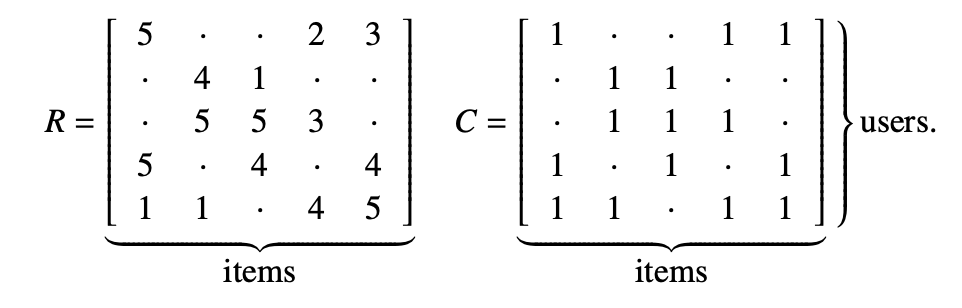
\includegraphics[width=0.75\linewidth]{images/R_C.png}
    \caption{User-item interaction matrices (R=ratings, C=interactions)}
    \label{fig:rc}
\end{figure}

Our next question is, “How to extract the necessary features from the user-item interactions without knowing or observing them?”, which is essentially the goal of \textbf{Matrix Factorization}, which looks for the underlying low-dimensional structure that explains these observations. 

Figure \ref{fig:mf} shows the goal of approximating a partially observed matrix in terms of lower-dimensional factors. We assume that $R_{|U|\times|I|}$ can be expressed as the matrix product of a tall matrix $\gamma_U$ and a fat matrix $\gamma_I$, such that the individual entries in $R_{u,i}$ can be estimated by taking the dot product of the corresponding row of $\gamma_U$ and the column of $\gamma_I$., i.e. $R_{u,i} = \gamma_U \cdot \gamma_I$. Here, $\gamma_U$ and $\gamma_U$ are vectors that represent the latent factors describing the user $u$ and item $i$ respectively. We can think of $\gamma_U$ as the features that represent the preferences of the user $u$ and $\gamma_I$ as the features that describe the item $i$. Hence, $u$ will have a high interaction with $i$ if they have compatible features.
Figure \ref{fig:ui_vectors} depicts such vectors.

\begin{figure}
    \centering
    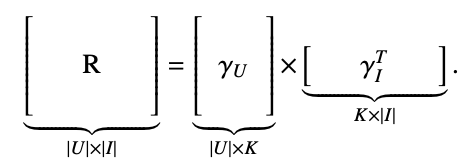
\includegraphics[width=0.75\linewidth]{images/SVD.png}
    \caption{Factorization of the user-item interactions matrix R}
    \label{fig:mf}
\end{figure}

\begin{figure}[h]
    \centering
    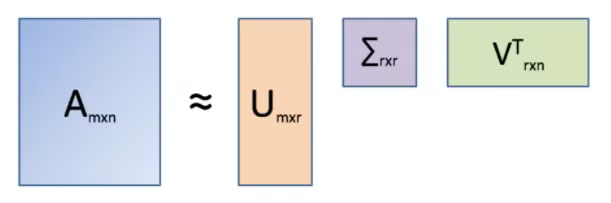
\includegraphics[width=0.75\linewidth]{images/image2.png}
    \caption{Singular Value Decomposition}
    \label{fig:svd}
\end{figure}

\begin{figure}[h]
    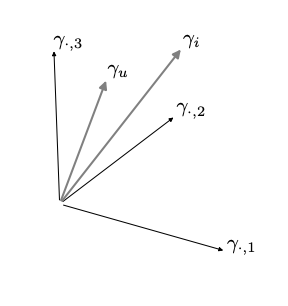
\includegraphics[width=0.4\linewidth]{images/ui_vectors.png}
    \caption{Representation of user $u$ and item $i$ in latent factor model}
    \label{fig:ui_vectors}
\end{figure}

This process of matrix factorization is strongly related to the SVD technique. The SVD of a real-valued matrix $M$ is given by $M=U \Sigma V^T$, where $U$ and $V$ are left and right singular values of $M$ (eigenvectors of $MM^T$ and $M^T M$), and $\Sigma$ is a diagonal matrix of eigenvectors of $MM^T$ (or $M^T M$). Critically, the best low-rank approximation of $M$ (say rank=K, in terms of the mean squared error) is found by taking the top K eigenvectors/eigenvalues in $U$, $\Sigma$ and $V$ (Eckart- Young theorem). If $u_i$s are the columns of $U$, $\sigma_i$s are the diagonal values in $\Sigma$, and $v_i^T$s are the rows of $V^T$, then

$M_k = \sum_{i=1}^{k} \sigma_i u_i v_i^T \quad , \sigma_1 \ge \sigma_2 \ge .. \ge 0$

\subsection{Approach description}
\textbf{TBD: We bring in BPR here and review with Joel...}

\subsection{SOTA approach description}

% \begin{figure}[h]
% \centering
% \begin{minipage}{.5\textwidth}
%   \centering
%   \includegraphics[width=.9\linewidth]{image5.png}
% \end{minipage}%
% \begin{minipage}{.5\textwidth}
%   \centering
%   \includegraphics[width=.9\linewidth]{image6.png}
% \end{minipage}
% \end{figure}


\section{Experiments}
\subsection{Setup and logistics}
\begin{itemize}
    \item We use Python as the programming language for this project. We will use Google Colab to develop the code and use GitHub for version control.
    \item We load the data from the HuggingFace dataset repository, and use several data-science libraries. We will use functions and APIs from NumPy, Pandas, Matplotlib, Surprise \cite{surprise}, Implicit \footnote{https://github.com/benfred/implicit}, PyTorch, and Transformers.
    % WordCloud, and Umap are used for graphs and visualization. 
    \item 
\end{itemize}

\subsection{Dataset and programming}

Let us see the implementation in code:

% \begin{lstlisting}[language=Python ]
% # necessary imports
% import numpy as np
% import pandas as pd
% import pprint
% pp = pprint.PrettyPrinter(indent=4)
% from tqdm.notebook import tqdm
% import matplotlib.pyplot as plt
% import seaborn as sns

% from sklearn.decomposition import TruncatedSVD
% from sklearn.feature_extraction.text import CountVectorizer
% from sklearn.feature_extraction.text import TfidfVectorizer
% from sklearn.datasets import fetch_20newsgroups

% from nltk.tokenize import word_tokenize
% from nltk.stem.porter import PorterStemmer
% from nltk.corpus import stopwords
% from nltk.stem import WordNetLemmatizer
% from wordcloud import WordCloud

% import warnings
% warnings.filterwarnings('ignore')
% \end{lstlisting} 

\subsection{Results}

\subsection{SOTA Results}

\subsection{Compare and contrast}
\begin{itemize}
    \item
\end{itemize}


\section{Conclusion}
\begin{itemize}
    \item This project covered the problem of recommendation systems
    \item We implemented SVD as a way to extract latent feature represenations of users and items from the latent matrix factorization of the user-item interaction matrix.
    \item In the project, we used the Amazon-Reviews-2023 dataset.
    \item We used data science libraries with Python to develop our code on Google Colab and used GitHub for version control.
    \item Finally, we saw the shortcomings of the standard SVD, and explored two better solutions using Bayesian probabilistic model and Transformers.
\end{itemize}

\section{Acknowledgement}
We are grateful to Prof. Tsui-Wei Weng, Halıcıoğlu Data Science Institute, San Diego and the TAs for their continuous support, encouragement, and willingness to help us throughout this project.

\bibliographystyle{abbrv}
\bibliography{references}

\end{document}